% !TEX spellcheck = uk_en
\documentclass[main.tex]{subfiles} 

\begin{document}

\section{Introduction}
\label{sec:1}

Currently, data produced from simulations and experiments is ever increasing 
in size and complexity. As computers become faster and more 
(fast) memory becomes available, data generation increases in tact with the technological 
advances. Scientists often produce terabytes\footnote{A house hold computer or desktop has a 
portion of this capacity as total storage.} of data from "simple" simulations. In order to process 
this data several approaches can be made. The data can be stored on a hard disk drive and 
thereupon accessed from any program. Users can either create their own software to process 
the data, or use prebuilt software intended for post processing. Depending on the complexity of the data, 
such software will have it's limitations. Software engineers and computer scientists often require 
specific features which suite their needs. A promising language like Python is becoming increasingly popular. 
It is an object-oriented language which offers an almost mathematical stylistic code. This
makes code readability that much easier for someone with a natural science background. 
Even though Python is an interpreted language, it is still possible to match languages such 
as Fortran and C in computational speed. Cython\footnote{\url{http://cython.org/}} provides the 
possibility to combine the efficiency of C with the ease of readability of Python. This combination 
is quite potent, as the computer scientist can possess the speed and still maintain few lines 
of code with mathematical tones.
\\

Our goal for this thesis will be to study and employ 
methods specifically for visualization of tensor fields. In general, this implies that given some 
data (regardless of it's dimension and order) how can we portray the data in such a way that 
the human mind can perceive it logically with as little effort as possible? Perception of complex 
structured data is the driving force behind this thesis. The challenge here lies in finding intuitive 
ways of visualizing data when the order or rank of the tensor increases. However, as the order of the tensor
increases so does the difficulty in our ability to visualize and interpret the data. As such we have 
choosen to limit ourselves to second order tensors in $\mathbf{R}^2$ and $\mathbf{R}^3$. 
Instead we focus on applying visualization techniques on a variety of data structures (this is not a trivial 
task to accomplish!). In order to visualize the results, we have created our own software.
\\

There are three common data structures : \textbf{scalar}, \textbf{vectorial}, and \textbf{tensorial}. 
Scalar data can often be visualized by employing color. For example, temperature and pressure can 
be visualized where the red color entails high values, and blue color low values. Every other value 
falls in between these colors; see for example Figure \ref{fig:nasa_temp}. As to the question : 
why exactly these colors? The apparent use of these colors stem from psycological 
reasonings. If someone desires to use an opposite color scheme, there are no restrictions to
visualize high and low values with the aforementioned color gambit. As a matter of fact,
it simply comes down to personal choices that an individual might find aesthetically pleasing.
As such, technically speaking, there are no limitations, but some standards do exist.
\begin{figure}
\hspace{35mm}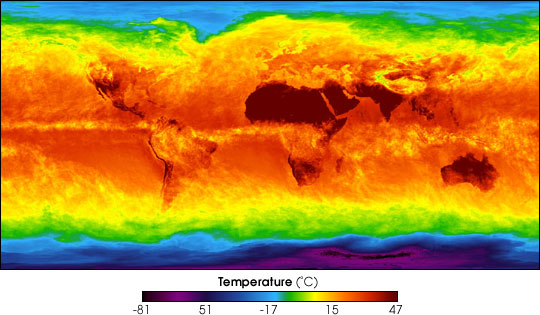
\includegraphics[scale=0.55,natwidth=540,natheight=315]{../figures/temperature_nasa.jpg} 
\caption[Color map of temperatures of Earth.]
{Picture taken from NASA Earth Observatorium.\footnotemark}
\label{fig:nasa_temp}
\end{figure}
\footnotetext{Source : \url{http://earthobservatory.nasa.gov/IOTD/view.php?id=3505}}

Often the scalar values are mapped to a color model. Given some data, we can 
assign each value to a specific color through a mapping function between a color model and a 
reference color space. Among some well known color maps are Jet, Parula\footnote{Which is the 
current default color map in Matlab.}, and Gray. Another color map is Viridis. Viridis has been 
developed for Python and has recently been added to Matplotlib as the default color map 
(intended for the release of version 2.0 \footnote{\url{http://matplotlib.org/style_changes.html}}).

Some color models which are worth mentioning :
\begin{itemize}
\item Computer monitors employ the sRGB model. The three primary colors red, green, 
and blue are used to reproduce an array of colors. Unlike the standard RGB model, sRGB also 
defines a nonlinear transformation between the intensities of the three colors and the number 
stored.
\item The CMY is a subtractive model, which uses the three primary colors cyan, magneta and
yellow. This color model is often employed by printers.
\item HSL and HSV are cylindrical coordinates representations of points in a RGB model. HSL
stands for hue, saturation, and lightness. While HSV stand for hue, saturation, and value.
Hue and saturation models are often used in image analysis. As such they are important models 
to be aware of.
\end{itemize}
Other techniques for 2D scalar data include \emph{contour curves}, which are often used in carthography
to display height differentials above for example sea level of similar values. For 3D scalar data similar 
techniques are used, with planes cutting through equal values, called \emph{isosurfaces}.
\\

For vectorial data in $\mathbf{R}^2$ and $\mathbf{R}^3$, an arrow entails to the length and 
direction of the data. Such data can be velocity and 
rotation for fluid flow, direction and strength of a magnetic field, or gradient of a scalar 
field (for a differentiable scalar function; e.g. temperature field). This is also referred
to as glyph-based technique. Depiciting such data with glyphs can quickly lead to clutter 
or occlusion of the field view. As such, glyph-based techniques are best suited for small 
datasets. We can also use field lines or path lines, to visualize the flow of a vector field. 
These flows often reveal the orientation of the field itself.
Again, the amount of data limits the use of such techniques. Another issue lies in guessing
proper seed points to extract important features. This is not an easy task if the properties of 
the field are unknown. One way to circumvent the problem of seeding and clutter is to use the LIC 
method\cite{CL93}. LIC stands for line integral convolution. This technique involves 
convoluting the vector field onto some noisy data. This generates dense visualization of the 
field lines along the vectors.
\\

Tensorial data can be of any order. In fact, scalar values are considered zeroth-order tensors, 
while vectors are considered to be first-order tensors (given that certain criterias are met, 
which we will discuss later in Chapter \ref{sec:2}). In this thesis we will focus on second-order 
tensors in $\mathbf{R}^2$ and $\mathbf{R}^3$. Such data can include stress and strain 
tensors, diffusion tensor for magnetic resonance (DT-MRI) in medical imaging, metric 
tensors in differential geometry, Reynolds-stress tensor for modelling turbulence, and 
many other tensor fields. As such, we have a diverse amount of physical problems we 
can visualize, even though we are limiting ourselves to second rank tensors.

We provide a quick reference over some of these tensors in Chapter \ref{sec:3}.


\vspace{5mm}Before we start discussing and dwelling deeper in the field of visualization of
tensor fields, a review is required of basic theory underlying tensors.
In order to understand tensors and their visualization, the 
reader needs to be familiar with vector and matrix operations (see Appendices 
\ref{sec:vis_vec_field} and \ref{sec:eigdecomp}). In Chapter \ref{sec:2},
we will focus on the underlying theory for tensor fields. In Chapter \ref{sec:3} the 
current research in the field of visualization of tensor fields is explored. In  
Chapter \ref{sec:4}, we divert our attention to the implementation of software for
various visualization methods. The results are portrayed and discussed in Chapter 
\ref{sec:5}. The final section, Chapter \ref{sec:6}, contains various conclusions
we draw based upon the findings from Chapter \ref{sec:3} and Chapter \ref{sec:5}.
All the relevant code listings are found in the Appendix \ref{sec:codelistings}.

The source code has been made accessible on the following repository : \url{https://github.com/imranal/DiffTens}.

\end{document}